\section{Theorie}
\label{sec:Theorie}


\subsection{Halbleiter}

\begin{figure}
    \centering
    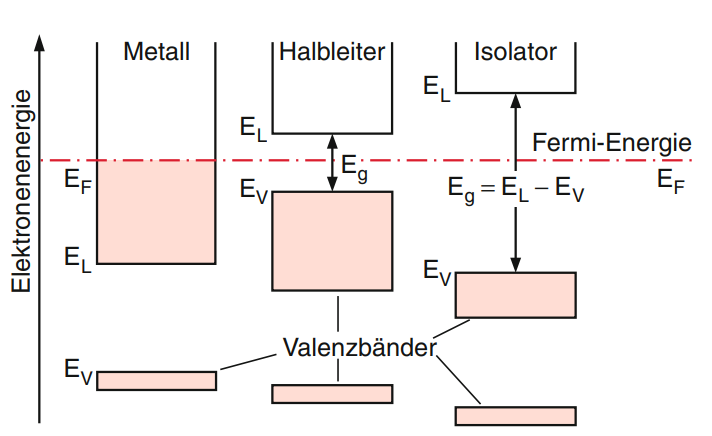
\includegraphics[width=.9\textwidth]{Bilder/Metall_Iso_Halb.PNG}
    \caption{Schematische Darstellung der jeweiligen Bandstrucktur von Metallen, Halbleitern und Isolatoren. \cite[S. 446]{Dem3}}
    \label{fig:band}
\end{figure}


Atome können sich über kovalente Bindungen zu Kristallen ordnen.
Aufgrund der hohen Anzahl an Atomen und deren gegenseitiger Wechselwirkung spalten sich die ursprünglich diskreten Energiezustände in sogenannte Bänder auf.
Je nach Größe und Position der Bandlücke lassen sich drei Arten von Materialien unterscheiden.
In Abbildung \ref{fig:band} sind die Bandschemata von Leitern, Halbleitern und Isolatoren dargestellt.
Die Energiezustände des niedrigeren Bandes (Valenzband) sind bei einer Temperatur $T=\SI{0}{\kelvin}$ vollständig bis zur Fermienergie gefüllt.
Diese Valenzelektronen, welche signifikant von dem Gitterpotential beeinflusst werden, dienen den kovalenten Bindungen zwischen den Atomen. 
Abgesehen von dem Leiter sind die Zustände des nächst höheren Bandes (Leitungsband) unbesetzt. 
Beim Leiter oder bei höheren Temperaturen können diese Zustände besetzt werden, in denen die besetzenden Elektronen nur kaum von dem Gitterpotential beeinflusst werden.
Deshalb sorgen diese freien Elektronen für die Leitfähigkeit des Materials. 
Der Hauptunterschied zwischen einem Isolator und einem Halbleiter ist die Größe der Bandlücke, welche bei dem Isolator deutlich über der Größenordung der thermischen Energie liegt.
Beim Halbleiter jedoch können Elektronen die Bandlücke mithilfe thermischer Energie überwinden.
Bei Halbleitern führt eine Erhöhung der Temperatur zu einer Erhöhung der Ladungsträgerdichte und damit einer erhöhten Leitfähigkeit.



Neben der Temperatur lässt sich die Leitfähigkeit von Halbleitern über Zufuhr von Fremdatomen verändern.
Diese Zufuhr wird Dotierung genannt.
Dabei können Atome verwendet werden, die nach vollständiger Bindung im Gitter, ein Elektron spendieren (Donator) oder selbst binden (Akzeptor). 
Ein Halbleiter, der mit Donatoren dotiert ist, wird als n-dotiert bezeichnet und ein Halbleiter, der mit Akzeptoren dotiert ist, wird p-dotiert genannt.
Über diese Veränderung der Ladungsträgerdichte lässt sich die Größe der Bandlücke manipulieren. 
In Abbildung \ref{fig:ak_don} sind die jeweiligen Bandlücken dargestellt.
Es sind nun auch bei einer Temperatur von $T=\SI{0}{\kelvin}$ Zustände im Leitungsband besetzt.

\begin{figure}[!ht]
    \centering
    \subfloat[][Bandlücke eines n-dotierten Halbleiters.]{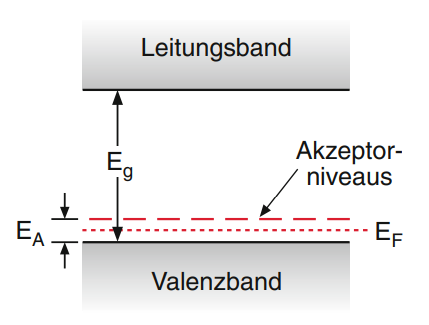
\includegraphics[width=.5\textwidth]{Bilder/Akzeptor.PNG}} 
    \subfloat[][Bandlücke eines n-dotierten Halbleiters.]{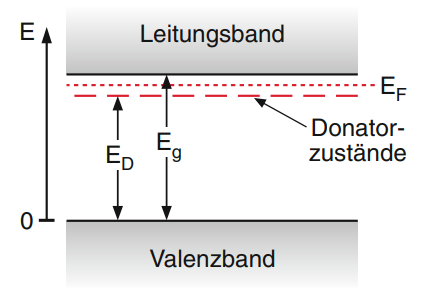
\includegraphics[width=.5\textwidth]{Bilder/Donator.PNG}}
    \caption{Darstellung der Bandlücken bei jeweiliger Zufuhr von Akzeptoren oder Donatoren. \cite[S. 453]{Dem3}}
    \label{fig:ak_don}
\end{figure}


\subsection{Effektive Masse}

Wie bereits oben erwähnt, können die Elektronen des Leitungsbandes als freie Ladungsträger bezeichnet werden.
Damit Gesetze der freien Elektronen auch auf die quasifreien Valenzelektronen angewandt werden können, wird eine effektive Masse eingeführt, welche die Wirkung des Gitterpotentials mit berücksichtigt.
Die effektive Masse lässt sich über
\begin{equation}
    m^* = \hbar^2 \left( \frac{\text{d}^2E(k)}{\text{d}k_i \text{d}k_j} \right)^{-1}
\end{equation}
definieren.
Somit ist diese proportional zur inversen Krümmung der Dispersionrelation.
Da der Kristall im Allgemeinen nicht isotrop ist, besitz die effektive Masse den Charakter eines Tensors, wodurch der Richtungsabhängigkeit Rechnung getragen wird.
Bei Kristallen hoher Symmetrie, wie es zum Beispiel bei dem im Versuch verwendeten GaAs der Fall ist, kann die Richtungsabhängigkeit vernachlässigt werden ($i=j$).



\subsection{Doppelbrechung}

\begin{figure}
    \centering
    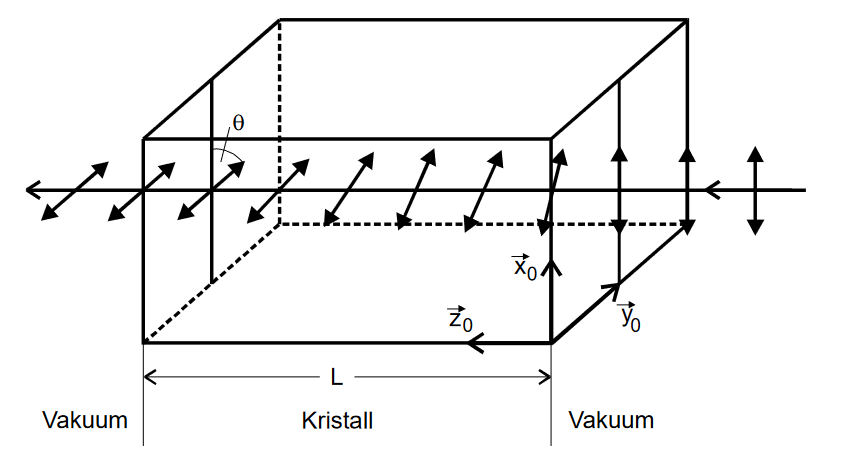
\includegraphics[width=.9\textwidth]{Bilder/Farad_Rot.PNG}
    \caption{Veranschaulichung der zirkularen Doppelbrechung bzw. der magnetfeldinduzierten Faraday Rotation. Die Polarisationsebene einer linear polarisierte Lichtwelle wird in einem Medium gedreht. \cite{V46}}
    \label{fig:farad_rot}
\end{figure}



\label{sub:doppel}
Optisch aktive Medien können aufgrund ihrer doppelbrechenden Eigenschaften die Polarisationsebene von linear polarisierten Licht um einen Winkel $\Theta$ drehen (siehe Abbildung \ref{fig:farad_rot}).
Jedes linear polarisierte Licht lässt sich als Superposition aus zwei jeweils entegengesetzt zirkular polarisierten Lichtwellen auffassen:
\begin{equation*}
    E(z) = \frac{1}{2} (E_R(z)+E_L(z)).
\end{equation*}
Es gelte für die jeweiligen Wellenvektoren $k_R \neq k_L$, lässt sich über Durchführung mehrerer Zwischenschritte der Drehwinkel über
\begin{equation}
    \Theta = \frac{L}{2}(k_R-k_L)
\end{equation}
bestimmen. Dabei steht $L$ für die Strecke, die das Licht im Medium zurückgelegt hat.
Aus der Relation zwischen Phasengeschwindigkeit und Wellenvektor
\begin{equation*}
    v = \frac{\omega}{k}
\end{equation*}
und der Beziehung zwischen Phasengeschwindigkeit und Brechungsindice
\begin{equation*}
    n = \frac{c}{v}
\end{equation*}
lässt sich der Drehwinkel auch über
\begin{equation}
    \Theta = \frac{L\omega}{2c}(n_R-n_L)
\end{equation}
berechnen. $c$ ist dabei die Lichtgeschwindigkeit im Vakuum und $\omega$ die Kreisfrequenz der Welle.




Die zirkulare Doppelbrechung entsteht durch elektrische Dipolmomente im Kristall.
In Summe wird dadurch eine makroskopische Polaristion $\vec{P}$ induziert, die bei geringem E-Feld der Gleichungen
\begin{equation*}
    \vec{P} = \epsilon_0 \chi \vec{E}
\end{equation*}
entspricht.
$\epsilon_0$ steht für die Influenzkonstante und $\chi$ für die dielektrische Suszeptibilität.
Im Allgemeinen ist $\chi$ ein Tensor, da Kristalle anisotrop sein können.
Die Drehung der Polarisationsebene entsteht durch eine Richtungsabhängigkeit der Brechungsindices. 
Links- und rechtspolarisierte Wellen erfahren jeweils unterschiedliche Brechungsindices und besitzen deshalb unterschiedliche Phasengeschwindigkeiten.
Trifft die linear polarisierte Welle auf ein doppelbrechendes Medium, laufen die jeweiligen Phasen der zirkularen Teilwellen auseinander.
In Summe äußert sich diese Dephasierung in einer Drehung der ursprünglichen Polarisationsebene.


\subsection{Faraday Rotation}
Tritt linear polarisiertes Licht durch ein optisch inaktives Medium, in dem ein zur Ausbreitunsrichtung paralleles Magnetfeld angelegt ist, wird die Polarisationsebene um einen Winkel $\Theta$ gedreht.
Dieser Effekt ist dem aus Abschnitt \ref{sub:doppel} verwandt und wird als Faraday Rotation bezeichnet.
Schließlich lässt sich der Drehwinkel über
\begin{equation}
    \label{theta}
    \Theta = \frac{e_0^3}{8\pi^2\epsilon_0c^3(m^*)^2}\lambda^2\frac{NB}{n} \cdot L
\end{equation}
berechnen.
Dabei steht $e_0$ für die Elementarladung, $\epsilon_0$ für die Influenzkonstante, $c$ die Lichtgeschwindigkeit,
$m^*$ die effektive Masse, $\lambda$ die Wellenlänge des Lichtes, $N$ die Donatorkonzentration,
$B$ die Magnetfeldstärke, $L$ die Probendicke und $n$ der Brechungsindex.
%In knapper Form sind die physikalischen Grundlagen des Versuches, des Messverfahrens, sowie sämtliche für die Auswertung erforderlichen Gleichungen darzustellen. (Keine Herleitung)

%(eventuell die Aufgaben)

%Der Versuchsaufbau: Beschreibung des Versuchs und der Funktionsweise (mit Skizze/Bild/Foto)
